%!TEX root = TQFTnotes.tex
%%%%%%%%%%%%%%%%%%%%%%%%%%%%%%
\chapter{2-categories}\label{c:2categories}

In the previous chapters, we classified all 2d TQFTs; the key step of this
classification was the fact that any cobordism can be obtained by composing a
small set of generating cobordisms (cup, cap, pants, copants). However, for
higher dimensions, this approach becomes hard; even for $n=3$, it is impossible
to produce a finite set of generating cobordisms.

A possible way out is rethinking the very idea of a cobordism. After all, the
initial physical motivation for TQFT was coming from path integral formulation,
which shows that the invariant of a closed $n$-manifold can be computed by
cutting the manifold into small local pieces, computing the path integral over
each of them (with appropriate boundary conditions) and summing up. Thus, we
just need to  formalize the idea of ``gluing the manifold from local pieces''.
For this, the notion of a cobordism is not enough.

One possible way of defining ``local pieces'' is using the notion of a manifold
with corners. For $n=2$, such a manifold could look like the one shown below:

%% definition of 2-category of bordisms
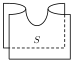
\includegraphics{figures/c7-fig01.svg}

This is a manifold with corners; you can think of it as a cobordism from the
union of two arcs at the top to the union of two intervals at the bottom. Each
of them is not a closed manifold but a 1d cobordism. Thus, for 2-dimensional
TQFT,  we have a structure where we have
\begin{itemize}
  \item 0-dimensional manifolds (corners)
  \item 1-dimensional cobordisms between them
  \item 2-dimensional cobordisms between 1d cobordisms
\end{itemize}

The appropriate language for describing this kind of structures is the
language of 2-categories. In this chapter, we give an overview of the theory
of 2-categories; we refer the reader to \cite{leinster} for details.

%%%%%%%%%%%%%%%%%%%%%%%%%%%%%%%%
\section{Strict 2-categories}\label{s:2cat-strict}
\begin{predefinition}\label{d:2-cat-prelim}
  A 2-category is the following collection of data:
  \begin{enumerate}
    \item A class $\calC_0$, called objects of $\calC$.
    \item For any $X,Y\in \calC_0$, a set $\Hom_{\calC}(X,Y)$,
    called 1-morphisms of $\calC$.
    \item For any pair of 1-morphisms $f,g\in \Hom_\calC(X,Y)$, a set
      $\Hom^2_{\calC}(f,g)$; elements of this set are called
      2-morphisms of $\calC$.
    \item Appropriate composition laws and identity morphisms for 1-
      and 2-morphisms.
  \end{enumerate}
\end{predefinition}
Before giving the full definition, here are the motivating examples ---
whatever definition we give, it must cover these examples (possibly with minor
technical modifications).

\begin{example}\label{x:cat}
  The 2-category $\cat$ of all (small) categories. Objects of this category are
  categories, 1-morphisms are functors, and 2-morphisms are functorial
  morphisms.
\end{example}
\begin{example} \label{x:alg}
  The 2-category $\Alg$ of algebras and bimodules. Objects of this category are
  unital associative algebras (not necessarily finite-dimensional) over a fixed
  ground field $\kk$, 1-morphisms $M\colon A\to B$ are $B$-$A$-bimodules,
  and 2-morphisms are morphisms of bimodules. Composition of 1-morphisms
  is given by tensor product over the algebra:
  $$
  ({}_CM_B, {}_BN_A)\mapsto {}_C M\otimes_B N_A
  $$
  (we use subscripts such as ${}_BN_A$ to indicate that $N$ is a left module
  over $B$ and a right module over $A$.)

  The identity 1-morphism from $A$ to $A$ is $A$ itself considered as an
  $A$-bimodule.
\end{example}
\begin{example} \label{x:2groupoid}
  Let $X$ be a topological space. Define its \emph{fundamental
  2-groupoid}\index{fundamental 2-groupoid} $\Pi_{\leq 2}(X)$ to be the
  following 2-category:
  \begin{itemize}
    \item Objects: points $x\in X$
    \item 1-morphisms: paths $\ga\colon I \to X$ between points
    \item 2-morphisms: equivalence classes of homotopies between paths
          (two homotopies are equivalent if there is a ``homotopy between
          homotopies'' between them)
  \end{itemize}
\end{example}

Morphisms and 2-morphisms in a 2-category are frequently presented graphically.
There are two approaches to it:
\begin{enumerate}
  \item Objects are represented by points, 1-morphisms by arrows,
    and 2-morphisms by 2-cells. This is the more common way.

  \item Objects are represented by regions in the plane, 1-morphisms by lines
    separating these regions (``domain walls''),
    and 2-morphisms by points where these lines meet (or by boxes).
    This approach is very familiar to physicists.
\end{enumerate}

Following \cite[Appendix A.4]{schommer-pries}, we will call diagrams of the
first kind \emph{pasting diagrams} and diagrams of the second kind \emph{string
diagrams}. In both cases, we will accept the convention that 1-morphisms go
``from left to right'', and 2-morphisms go ``from top to bottom''. The figure
below (borrowed with modifications from \cite{schommer-pries}) shows a
comparison of these two types of graphical presentation.

\begin{figure}[ht]
  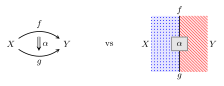
\includegraphics{figures/c7-fig02.svg}
  \caption{Pasting Diagrams vs String Diagrams}
\end{figure}

To turn \deref{d:2-cat-prelim} into a rigorous definition, we need to
define compositions for 1-morphisms and 2-morphisms and state appropriate
associativity and unit laws. There are a couple of subtle points; for
example, for 2-morphisms we need not only composition of 2-morphisms
shown below (vertical composition)
\begin{figure}[h]
  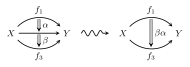
\includegraphics{figures/c7-fig03.svg}
\end{figure}

\noindent
but also ``horizontal composition'', which we denote by $\be\ccirc \al$
to distinguish it from the vertical composition:
\begin{figure}[h]
  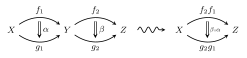
\includegraphics{figures/c7-fig04.svg}
\end{figure}

We can save some effort if we start by saying that for given objects
$X,Y$, all 1-morphisms between them, together with 2-morphisms between those,
form a category. That takes care of (vertical) composition of 2-morphisms,
identity 2-morphism, etc.

\begin{definition}\label{d:2-cat-strict}\index{2-category!strict}
  A strict 2-category $\calC$ is the following collection of data:
  \begin{itemize}
    \item A class of objects $\calC_0$
    \item For any $X, Y\in \calC_0$, a category $\Hom_{\calC}(X,Y)$. Objects of
      this category are called $1$-morphisms from $X$ to $Y$; morphisms
      of $\Hom_{\calC}(X,Y)$ are called $2$-morphisms of $\calC$
    \item A (horizontal) composition functor
      $$
        H\colon \Hom(X,Y)\times \Hom(Y,Z)\to \Hom(X,Z)
      $$
    \item For every $X\in \calC$, an identity 1-morphism $1_X\in \Hom(X,X)$
  \end{itemize}
  such that the horizontal composition is associative and $1_X$ is a unit
  for this composition.
\end{definition}
Instead of providing a $1$-morphism $1_X\in \Hom(X,X)$, we can say
``we have a functor $\one\to\Hom(X,X)$'', where $\one$ is the category
with a single object and a unique morphism (namely, the identity morphism).

Note that since composition is a functor, it also gives a horizontal
composition of 2-morphisms; thus, this is automatically taken care of --- no
need to add horizontal composition of 2-morphisms by hand.

The exact meaning of ``horizontal composition is associative'' is as follows.
For any $X,Y,Z,W\in \calC$, one can construct two functors
$$
\Hom(X,Y)\times \Hom(Y,Z)\times\Hom(Z,W)\to \Hom(X,W)
$$
namely, $H\circ (H\times \id)$ and $H\circ (\id \times H)$. Associativity
means that these two functors are equal. Similarly one can write down the exact
meaning of ``$1_X$ is a unit for horizontal composition''.

\begin{exercise}\label{ec:exchange_condition}
  Consider the pasting diagram below. Then there are two obvious ways to
  compose the four 2-morphisms in this diagram into a single 2-morphism from
  $f_2f_1$ to $g_2g_1$: either using horizontal composition first or using
  vertical composition first. Prove that the resulting 2-morphisms are equal.

  \begin{figure}[h]
    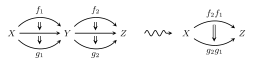
\includegraphics{figures/c7-fig05.svg}
  \end{figure}
  This is known as the ``exchange condition''; it is a special case of the
  so-called \emph{pasting theorem}; broadly speaking, this theorem claims that given a
  composable pasting diagram, the result of composition does not depend on the order
  in which we are doing the compositions. Formulating it precisely is somewhat
  technical; see \cite{power-pasting}.
\end{exercise}
\begin{lemma}\label{l:eckmann-hilton}
  Let $X$ be an object in a strict 2-category $\calC$. Consider the monoid of
  2-morphisms $\Hom(1_X, 1_X)$. Then horizontal and vertical compositions
  coincide, and the resulting composition is commutative.
\end{lemma}
This is known as the \emph{Eckmann--Hilton argument}\index{Eckmann--Hilton argument}; see
\cite[Lemma 1.2.4]{leinster}. It can be viewed as a categorical analog of
the well-known topological fact: for $k>1$, homotopy groups $\pi_k(X)$
are commutative.

\begin{exercise}\label{ec:algebra-in-2cat}
  Let $A$ be an associative algebra, considered as an object in the 2-category
  $\Alg$. Prove that then $\Hom_{\Alg}(1_A, 1_A)=z(A)$ is the center of $A$.
\end{exercise}
%%%%%%%%%%%%%%%%%%%%%%%%%%%%%
\section{Weak 2-categories}\label{s:weak-2cat}
There is one problem with the notion of strict 2-category: this definition is
too strict. For example, in the proposed 2-category of algebras and bimodules,
the identity 1-morphism $1_A\in \Hom(A,A)$ is $A$ considered as an $A$-bimodule.
But if $M$ is an $A$-$B$-bimodule, $A\otimes_A M$ is not equal to $M$: it is only
isomorphic. Thus, we need to relax the associativity condition for composition
of 1-morphisms, similarly to what we did with the associativity condition for
monoidal categories.

\begin{definition}\label{d:2-cat-weak}
  A \emph{weak 2-category}\index{weak 2-category} (also called a bicategory) $\calC$ is the following
  collection of data:
  \begin{itemize}
    \item A class of objects $\calC_0$
    \item For any $X, Y\in \calC_0$, a category $\Hom_\calC(X,Y)$. Objects of
      this category are called $1$-morphisms from $X$ to $Y$; morphisms of
      $\Hom_\calC(X,Y)$ are called $2$-morphisms of $\calC$
    \item A (horizontal) composition functor
      $$
        H\colon \Hom(X,Y)\times \Hom(Y,Z)\to \Hom(X,Z)
      $$
    \item For every $X\in \calC_0$, an identity 1-morphism $1_X\in \Hom(X,X)$
    \item For any quadruple of objects $X,Y,Z,W\in \calC$, an isomorphism
      $\al$ of functors $H\circ (H\times \id)$ and $H\circ (\id \times H)$,
      both considered as functors
      $$
        \Hom(X,Y)\times \Hom(Y,Z)\times\Hom(Z,W)\to \Hom(X,W).
      $$
    \item Left and right unit isomorphisms
  \end{itemize}
  which satisfy the pentagon and triangle axioms.
\end{definition}
The pentagon and triangle axioms are similar to those for a monoidal category;
details can be found, e.g., in \cite[Section 1.5]{leinster}.

\begin{example}\label{x:weak-2cat-examples}\par\noindent
  \begin{enumerate}
    \item The 2-category $\Alg$ of algebras and bimodules,
      introduced in \exref{x:alg}, is
      indeed a weak 2-category.
    \item The 2-category $\cat$ of (small) categories,
      introduced in \exref{x:cat}, is indeed a weak 2-category.
    \item As a variation of the above, we can define a weak 2-category $\ab_\kk$
      of $\kk$-linear abelian categories, together with $\kk$-linear functors
      between them. We can also impose some additional restrictions, such as
      local finiteness (all $\Hom$ spaces are finite-dimensional, and every
      object has finite length) or semisimplicity.
  \end{enumerate}
\end{example}
\begin{example}\label{x:BC}
  Let $\calC$ be a monoidal category. Define the 2-category $\calB\calC$ as the
  2-category with one object $*$ and morphisms given by $\Hom_{\calB\calC}(*,*)
  =\calC$, with horizontal composition given by tensor product.
  It is easy to see that this is indeed a 2-category;
  conversely, every 2-category with only one object is obtained in this
  way. This is sometimes called \emph{delooping}\index{delooping} of $\calC$.
\end{example}

\begin{remark}\label{r:BG}
    The notation $\calB\calC$ is motivated by the following. Let $M$ be a
    monoid (for example, a group). Define the category $\calB M$ as the
    category with a single object $*$ and $\Hom(*,*)=M$. Then it is immediate
    from the definition that for a group $G$, the so-defined category is
    equivalent to the fundamental groupoid of the classifying space $BG$:
    $\calB G\simeq \Pi_1(BG)$; therefore, $\calB$ is the categorical analog of
    the classifying space construction.

  The word ``delooping'' is justified by the following observation: for a
  path-connected topological space $X$, let $\Omega X$ be the space of based
  loops in $X$. Then we have a homotopy equivalence $\Omega BG \simeq G$; thus,
  in some sense $B$ is the inverse operation to $\Omega$, hence the name
  ``delooping''.
\end{remark}

One can also define the notion of functor between (weak) 2-categories,
which we skip, referring the reader to \cite[Definition 1.5.8]{leinster}.
(Note: what we will be using is called ``weak lax functors'' in
\cite{leinster}.) This allows one to define the notion of equivalence of weak
2-categories.

\begin{theorem}\label{t:strictify-bicategories}
  Any weak 2-category is equivalent to a strict 2-category.
\end{theorem}
This theorem is similar to the coherence theorem \thref{t:strictify}; we refer
the reader to \cite[Theorem 1.5.15]{leinster} for the proof.

\begin{remark}\label{r:stictify-3-cat}
  Do not let this theorem give you the wrong idea. For $n=3$, the notion of a
  weak $3$-category (which is quite hard to define, see
  \cite{gordon-power-street}) is not equivalent to that of a strict 3-category
  (which is relatively easy to define). We will return to this when discussing
  higher categories in \chref{c:higher-cat}.
\end{remark}


\begin{convention}
  From now on, the name ``2-category'' will mean a weak 2-category unless
  explicitly stated otherwise.
\end{convention}
Note that it is easy to go from a 2-category to a 1-category.
\begin{definition}\label{d:hC}
  Let $\calC$ be a weak 2-category. Define the category $\tauone\calC$
  as follows:
  \begin{itemize}
    \item Objects of $\tauone\calC$ are the same as objects of $\calC$.
    \item Morphisms of $\tauone\calC$ are isomorphism classes of 1-morphisms in
    $\calC$
  \end{itemize}
  We will call $\tauone\calC$ the 1-truncation of $\calC$; it is also frequently
  called the  \emph{homotopy category}\index{homotopy category} of $\calC$.
  Alternative notation for $\tauone\calC$ is $h\calC$.
\end{definition}

%%%%%%%%%%%%%%%%%%%%%%%%%%%%%
\section{Symmetric monoidal 2-categories}\label{s:sym-mon-2cat}


Our next goal is defining the notion of a monoidal weak 2-category. We will
outline the construction but skip all the details, referring the reader to
\cite[Appendix C]{schommer-pries}.

Throughout this section, $\calC$ is a weak 2-category.

As with a usual monoidal category, the starting point is a tensor product
functor $\otimes\colon \calC \times \calC \to \calC$. However, we need to define
what it means for $\otimes$ to be associative. To put it into perspective,
recall the notion of associativity at previous levels of complexity:
\begin{itemize}
  \item when defining a monoid, we had a map of sets $M\times M \to M$
    and we required $a(bc) = (ab)c$
  \item when defining a monoidal category, we had a functor
    $\otimes\colon \calC\times \calC \to \calC$;
    the requirement $A\otimes (B \otimes C) = (A\otimes B) \otimes C$
    does not make sense (objects in a category are never
    equal), so instead we introduced the associativity isomorphism
    $\al \colon (A\otimes B)\otimes C \to A\otimes (B \otimes C)$ and
    imposed an extra consistency relation, the pentagon axiom (which
    comes from trying to identify all 5 possible
    ways of bracketing the tensor product of 4 objects)
  \item now, in a 2-category, we need to have the tensor product functor and
    the associativity isomorphism $\al$. But now each side of the pentagon axiom
    is a composition of 1-morphisms. By the same logic, it is meaningless to
    require that this diagram is commutative --- 1-morphisms in a 2-category are
    rarely equal, just isomorphic. Thus, we need to provide a 2-isomorphism
    $\pi$ between the two sides of the pentagon diagram; we will call it
    ``pentagrammator''.
  \end{itemize}

  \begin{equation}\label{e:pentagon-2cat}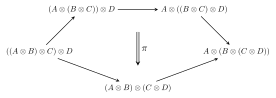
\includegraphics{figures/c7-fig06.svg}\end{equation}


The so-defined pentagrammator must itself satisfy some compatibility
conditions. Not surprisingly, it comes from a cell of dimension 3 in Stasheff's
associahedron $K_5$ (see \reref{r:stasheff}). Recall that  this polyhedron has
14 vertices, corresponding to 14 bracketings of the tensor product of 5
objects; edges of $K_5$  correspond to application of associativity
isomorphisms, and 2-cells correspond to  pentagon axiom and functoriality
relation. As discussed before, the MacLane coherence axiom for monoidal
categoires implies that the 2-skeleton of $K_5$ is simply-connected.  In fact,
it is homeomorphic to a 2-sphere: $K_5$ is topologically a 3-ball, and the
2-skeleton is the boundary of that ball.

We now add a relation corresponding to the single 3-cell in $K_5$;
this relation has the form
\begin{align*}
  &\text{(composition
  of 2-morphisms in the 2-cells in the upper hemisphere)}\\
  & \qquad =
  \text{(composition of 2-morphisms in the 2-cells in the lower hemisphere)}.
\end{align*}

This gives us a consistency relation for the pentagrammator 2-morphism, called
the \emph{associahedron} equation. To give you some idea of what it looks like,
\firef{f: associahedron} shows the pasting diagram for one side of the
associahedron equation, which corresponds to the upper hemisphere in the
14-vertex 3-cell. The lower side is similar. (This diagram is copied from
\cite[Appendix C]{schommer-pries}; he uses $a$ instead of $\al$ for the
associativity 1-morphism.)

\begin{figure}[ht]
\tikzset{l/.style={font=\fontsize{8}{8}\selectfont}}
   \begin{center}
       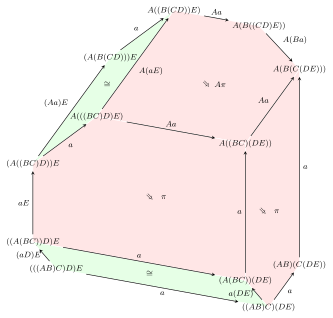
\includegraphics{figures/c7-fig07.svg}% End sketch output
	\end{center}
	\caption{Pasting diagram for the left-hand side of the associahedron axiom.
    Green 2-cells correspond to commutative diagrams given by functoriality.}
	\label{f: associahedron}
\end{figure}

In a similar way, instead of requiring the commutativity of diagrams involving
the left and right unit isomorphisms, we now need to introduce 2-morphisms
(``unitors'') filling these diagrams, and then impose additional relations on
them coming from 3-cells.

We will not be providing any details of this, referring the reader to
\cite{schommer-pries}. Instead, we will show some examples.


\begin{example}\label{x:alg-bimodules}
  Let $\Alg$ be the weak 2-category of algebras and bimodules as defined in
  \exref{x:alg}. Then it has a natural structure of a symmetric monoidal
  2-category, with $\otimes$ being the usual tensor product of algebras.
\end{example}

\begin{remark}
  Recall that a monoidal category $\calC$ is essentially the same as a
  weak 2-category $\calB\calC$ with one object. Similarly, a monoidal
  2-category is the same as a weak 3-category with one object; the
  associahedron equation is a special case of a consistency equation for
  associativity of composition of 1-morphisms in a 3-category.
\end{remark}


%%%%%%%%%%%%%%%%%%%%%%%%%%%%%%%
\section{Locally finite categories and Deligne product}
\label{s:deligne-product}
In this section, we give an example of a symmetric monoidal weak 2-category.
Namely, recall that a $\kk$-linear abelian category $\calA$ is called
\emph{locally finite}\index{category!locally finite} if
\begin{itemize}
    \item for any $X,Y\in \calA$, the space $\Hom_{\calA}(X,Y)$ is
      finite-dimensional, and
    \item every object $X\in \calA$ has finite length
\end{itemize}
(see \cite[Section 1.8]{etingof-fusion}). Denote by $\Linlf$ the 2-category
of locally finite $\kk$-linear abelian categories, with 1-morphisms given by
\emph{right exact} $\kk$-linear functors and 2-morphisms given by functorial
morphisms (some motivations for restricting ourselves to right exact
functors will be discussed in \chref{c:3cat-tens}). %FIXME


Our next goal is defining an analog of tensor product in $\Linlf$.
Let $\calC, \calD, \calE$ be $\kk$-linear categories. Denote by
$\Bil(\calC\times\calD, \calE)$ the category of $\kk$-bilinear functors $F\colon
\calC\times\calD\to \calE$ which are right exact in each of the arguments.

\begin{definition}\label{d:deligne-product}
  The Deligne product of $\kk$-linear categories $\calC$, $\calD$ is a
  $\kk$-linear category $\calC\boxtimes \calD$ together with a bilinear functor
  $\calC\times\calD\to \calC\boxtimes\calD$ such that for any $\calE$, we have
  an equivalence
  $$
    \Bil(\calC\times\calD, \calE)\simeq \Fun(\calC\boxtimes\calD, \calE).
  $$
  where $\Fun$ is the category of $\kk$-linear right exact functors.
\end{definition}
This definition mimics the definition of tensor product of vector spaces as a
universal object. As usual with such definitions, if such a category
$\calC\boxtimes\calD$ exists, it is unique: any two such categories are
canonically equivalent. However, existence is not obvious and in fact may fail
without some assumptions on $\calC$, $\calD$.

\begin{theorem}\label{t:deligne-product}\index{Deligne's product}
  If $\calC$, $\calD$ are locally finite categories,
  then $\calC\boxtimes \calD$ exists
  and is a locally finite $\kk$-linear category.
\end{theorem}
We refer the reader to \cite[Section 1.11]{etingof-fusion} for the proof of
this theorem as well as results below.
\begin{lemma}\label{l:deligne-product-mod}
  \begin{enumerate}
  \item
    For a finite-dimensional algebra $A$, denote by $A\mod$ the category of
    finite-dimensional left $A$-modules. Then
    $$
      (A\mod)\boxtimes (B\mod) \simeq (A\otimes B)\mod.
    $$
  \item
    For any objects $X_1, Y_1\in \calC$, $X_2, Y_2\in \calD$, we have a
    canonical isomorphism
    $$
       \Hom_{\calC \boxtimes \calD} (X_1\boxtimes X_2, Y_1\boxtimes Y_2 )\simeq
         \Hom_{\calC} (X_1,  Y_1) \otimes
         \Hom_{\calD} (X_2, Y_2 ).
    $$
  \item If $\calC$, $\calD$ are semisimple $\kk$-linear categories with simple
    objects $X_i, Y_j$ respectively, then $\calC\boxtimes \calD$ is also
    semisimple, with simple objects $X_i\boxtimes Y_j$.
   \end{enumerate}
\end{lemma}

\begin{theorem}\label{t:linear-monoidal-2cat}
  The 2-category $\Linlf$ is a symmetric monoidal 2-category, with tensor
  product functor given by Deligne's product $\boxtimes$ and unit given by the
  category $\vecf$.
\end{theorem}
We skip the proof, which is mostly straightforward; we just note that to show
that $\vecf$ is the unit for this monoidal structure, we need to construct,
for any $\calC\in \Linlf$, an equivalence of categories $\vecf\boxtimes
\calC\simeq \calC$.

Another way of stating this is by saying that any locally finite $\kk$-linear
category has a natural structure of a module category over $\vecf$ (we will
discuss the general notion of a module category later, in
\seref{s:module-categories}). Namely, for a
finite-dimensional vector space $V$ and an object $X\in \calC$ in a locally
finite category $\calC$, we define the object $V\otimes X$ by the condition that
for any object $Y\in \calC$, we have a canonical isomorphism
$$
  \Hom(Y, V\otimes X)=V\otimes \Hom(Y, X)
$$
(more formally, $V\otimes X$ is the object (co)representing the functor
$F(Y)=V\otimes \Hom(Y,X)$).

\clearpage
